\let\negmedspace\undefined
\let\negthickspace\undefined
\documentclass[journal]{IEEEtran}
\usepackage[a5paper, margin=10mm, onecolumn]{geometry}
\usepackage{tfrupee} 

\setlength{\headheight}{1cm}
\setlength{\headsep}{0mm}

\usepackage{gvv-book}
\usepackage{gvv}
\usepackage{cite}
\usepackage{amsmath,amssymb,amsfonts,amsthm}
\usepackage{algorithmic}
\usepackage{graphicx}
\usepackage{textcomp}
\usepackage{xcolor}
\usepackage{txfonts}
\usepackage{listings}
\usepackage{enumitem}
\usepackage{mathtools}
\usepackage{gensymb}
\usepackage{comment}
\usepackage[breaklinks=true]{hyperref}
\usepackage{tkz-euclide} 
\usepackage{listings}

\def\inputGnumericTable{}                                 
\usepackage[latin1]{inputenc}                                
\usepackage{color}                                            
\usepackage{array}                                            
\usepackage{longtable}                                       
\usepackage{calc}                                             
\usepackage{multirow}                                         
\usepackage{hhline}                                           
\usepackage{ifthen}                                           
\usepackage{lscape}

\title{\textbf{4.10.4}}
\author{\textbf{EE25BTECH11006 - ADUDOTLA SRIVIDYA}}
\date{september 15, 2025}

\begin{document}

\maketitle

Question:\\
Find the coordinates of the point where the line through the points $A(3,4,1)$ and $B(5,1,6)$ crosses the $XY$ plane.

\solution:\\
The equation of the line passing through:
\begin{align}
    \vec{A} = \myvec{ 3 \\ 4 \\ 1}, \quad
    \vec{B} = \myvec{5 \\ 1 \\ 6}
\end{align}
The direction vector of the line 
\begin{align}
    \vec{m} &= \vec{A} - \vec{B} \\
    &= \myvec{-2 \\ 3 \\ -5}
\end{align}
vector equation of the line is
\begin{align}
    \vec{x} = \vec{A}+\lambda\vec{m}
\end{align}
equation of $XY$ plane is
\begin{align}
    \myvec{0 & 0 & 1}\vec{x} = 0
\end{align}
Solving the equation of plane ($\vec{n}^{T}\vec{x}=0$) and the line ($\vec{x}=\vec{A}+\lambda\vec{m}$),
\begin{align}
    \vec{n}^{T}(\vec{A}+\lambda\vec{m})&=0\\
\vec{n}^{T}\vec{A}+\lambda\vec{n}^{T}\vec{m}&=0\\
\lambda&=\tfrac{-\vec{n}^{T}\vec{A}}{\vec{n}^{T}\vec{m}}\\
\end{align}
\newpage
\textbf{Substituting the $\vec{n},\vec{A},\vec{m}$}
\begin{align}
\lambda&=\dfrac{-\myvec{0\\0 \\1}^{T}\myvec{3\\4\\1}}{\myvec{0\\0 \\1}^{T}\myvec{-2\\3\\-5}}\\
&=\tfrac{-(0+0+1)}{0+0-5}\\
&=\tfrac{-1}{-5}\\
\lambda&=\tfrac{1}{5}
\end{align}
Therefore,
\begin{align}
    \vec{x} &= \myvec{3\\4\\1} + \myvec{\dfrac{-2}{5} \\ \dfrac{3}{5} \\ -1} \\
    &= \myvec{\dfrac{13}{5} \\ \dfrac{23}{5} \\ 0}
\end{align}
The point where the line crosses the $XY$ plane is :
\begin{align}
    \vec{x} = \myvec{\dfrac{13}{5} \\ \dfrac{23}{5} \\ 0}
\end{align}

\begin{figure}[H]
    \centering
    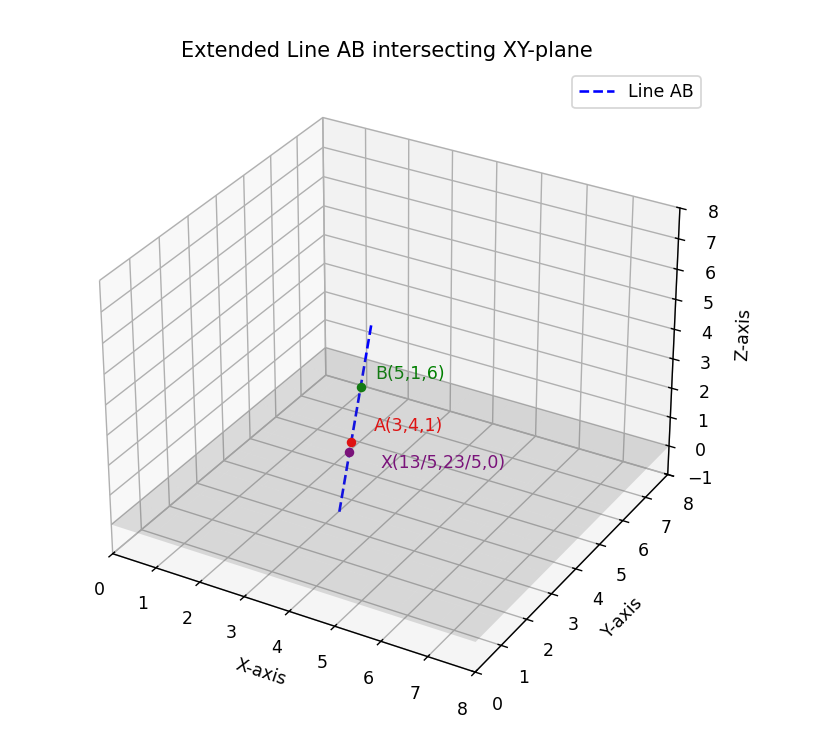
\includegraphics[width=0.8\linewidth]{figs/fig.png}
    \caption{Caption}
    \label{fig:placeholder}
\end{figure}

\end{document}